\documentclass[a4paper, 12pt]{article}

\usepackage[left=2cm,right=2cm,
    top=2cm,bottom=2cm,bindingoffset=0cm]{geometry}

\usepackage[T2A]{fontenc}
\usepackage[utf8]{inputenc}
\usepackage{color}
\usepackage{graphicx}
\usepackage{caption}
\usepackage{subcaption}
\usepackage{tikz}
\usepackage[english, russian]{babel}
\usepackage{ gensymb }
\usepackage{booktabs}
\usepackage{amsmath,amsfonts,amssymb,amsthm,mathtools}
\usepackage{lscape}

\begin{document}
\begin{center}
\textbf{\textit{Метод конечных элементов для одномерной задачи теплопроводности в стержне}}
\end{center}
\textbf{\textit{Задание.}} К закрепленному в стене концу стержня $(x=0)$ подводится тепловой поток интенсивности $q$. На свободном конце стержня $(x=L)$ происходит конвективный теплообмен тепла. Коэффициент теплообмена $h$, температура окружающей среды $T_{\text{ср}}$. Через боковую поверхность стержня также происходит конвективный теплообмен. Площадь поперечного сечения стержня $S$ считается постоянной.

Решить задачу методом конечных элементов с использованием одномерного линейного (симплекс) элемента. Выписать в тетради явное решение СЛАУ в случае когда стержень разбит на 3 элемента.

Разбить стержень на 5 конечных элементов и вычислить температуру в узлах МКЭ запрограммировав на языке С++.

\text{Решить задачу при следующих данных:} \\

$k_x = 75 \left[\frac{\text{Вт}}{(\text{см}) \cdot ^\circ \text{C}}\right]$ \quad - \text{коэффициент теплопроводности материала}, \\

$q = -150 \left[\frac{\text{Вт}}{\text{см}^2}\right]$ \quad (считается, что положительное направление, когда тепло отводится от тела, так как по задаче тепло подводится к телу, то знак минус), \\

$\alpha_g = 10 \left[\frac{\text{Вт}}{(\text{см}^2) \cdot ^\circ \text{C}}\right]$ \quad - \text{коэффициент теплообмена}, \\

$S = \pi \, \text{см}^2, \quad L = 7.5 \,$ \text{см}

\begin{center}
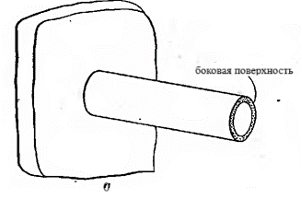
\includegraphics[width=0.4\textwidth]{pic.jpeg}
\end{center}

\begin{center}
\textbf{\textit{Решение}}
\end{center}

























\end{document}